\documentclass[conference]{IEEEtran}
\usepackage{amsmath,amsfonts}
\usepackage{algorithmic}
\usepackage{algorithm}
\usepackage[caption=false,font=normalsize,labelfont=sf,textfont=sf]{subfig}
\usepackage{textcomp}
\usepackage{stfloats}
\usepackage{url}
\usepackage{hyperref}
\usepackage{listings}
\usepackage{xcolor}
\usepackage{graphicx}
\usepackage{booktabs,threeparttable}
\hyphenation{op-tical net-works semi-conduc-tor IEEE-Xplore}
% updated with editorial comments 8/9/2021
\usepackage{biblatex}
\addbibresource{references.bib}


% Syntax highlighting
\definecolor{codegreen}{rgb}{0,0.6,0}
\definecolor{codegray}{rgb}{0.5,0.5,0.5}
\definecolor{codepurple}{rgb}{0.58,0,0.82}
\definecolor{codeorange}{rgb}{0.9,0.45,0.3}
\definecolor{backcolour}{rgb}{0.95,0.95,0.92}
\lstdefinestyle{cStyle}{
    language=C, % Identifiers from C
	alsoletter={\{,\}},
    commentstyle=\color{codegreen}, % Green comments, like we used to
    keywordstyle=\color{blue}, % Blue keywords like 'int'
    numberstyle=\tiny\color{codegray}, % Grey numbers
    numbers=left, % Line number on left side
    stringstyle=\color{codeorange}, % Strings look orange
    basicstyle=\ttfamily\footnotesize, % Same size for code as footnotes
    captionpos=t, % Caption on top
    xleftmargin=2em, % Margin on left side
    showstringspaces=false, % Don't show whitespaces
    tabsize=4, % Who doesn't use tabsize=4?
	emph=[1]{auto,break,case,char,const,continue,default,do, double, else, enum, extern, float, for, goto, if, int, long, register, return, short, signed, sizeof, static, struct, switch, typedef, union, unsigned, void, volatile, while, \{,\}},
    emphstyle=[1]{\color{codepurple}}, % Color keywords purple
    frame=lines, % Put the snippet within horizontal lines
}

\begin{document}

\title{An HTTP Server and RESTful API in Python}

\author{
	\IEEEauthorblockN{Fougeray Paul}
	\IEEEauthorblockA{
		\textit{Department of Computer Science } \\
		\textit{UiT The Arctic University of Norway}\\
		Tromsø, Norway \\
		pafou7668@uit.no
	}
}
\markboth{INF-2300 Assignment 1 \today}%
{An HTTP Server and RESTful API in Python}


\maketitle

\begin{abstract}
	This report presents an HTTP/1.1 server written in Python. I use the
	low-level \texttt{socketserver} module instead of a ready-made HTTP
	library. The server exposes a static file endpoint with \texttt{GET} and
	\texttt{POST}. It also exposes a RESTful \texttt{/messages} endpoint with
	\texttt{GET}, \texttt{POST}, \texttt{PUT} and \texttt{DELETE} on JSON
	resources. Messages persist to disk between restarts. The assignment
	leaves many edge cases open, so I document and justify my choices for
	them in this report. I verify the solution with an automated test suite
	and with Wireshark packet captures.
\end{abstract}

\begin{IEEEkeywords}
	HTTP, REST, socket programming, JSON, persistence.
\end{IEEEkeywords}

\section{Introduction}
\label{Section:Introduction}
The goal of this assignment is to understand HTTP by implementing it on raw
TCP sockets, instead of using a ready-made HTTP library. I then build a
small REST API on top of the same server. Working at this level makes
several hidden details explicit. I need to know where a request ends on the
wire. I need to know the body length in advance. I need to build a response
that a client can parse without ambiguity.

I use one generic request handler for both parts of the assignment: the
static file endpoint and the \texttt{/messages} REST endpoint. This follows
the assignment's advice to write a single server. Both parts share the same
parsing and response code. Only the routing step differs between them.

Much of this report explains and justifies my choices for the edge cases
the assignment leaves open. For example: what should happen on a
\texttt{PUT} request with no \texttt{id}? What should happen on a
\texttt{POST} to a message URL that already names a specific id?

\subsection{Outline}\label{Subsection:Outline}
The rest of this report is organized as follows. Section
\ref{Section:Theoretical Background} covers the background needed for the
rest of the report. Section \ref{Section:Design} gives a high-level view of
my design. Section \ref{Section:Implementation} explains my implementation
in detail. Section \ref{Section:Experiments and Results} describes my test
methodology and results. Section \ref{Section:Discussion} discusses the
design choices behind my handling of edge cases. Section
\ref{Section:Conclusion} concludes the report and lists possible future
work.


\section{Theoretical Background}\label{Section:Theoretical Background}

\subsection{HTTP message structure}\label{Subsection:http_structure}
An HTTP/1.1 message has a start-line, a set of header fields, a blank line,
and an optional body~\cite{rfc9112}. A connection can stay open for several
requests, so a server cannot read the body "until the socket closes": it
needs to know the body length in advance, before it can safely stop
reading and move on to the next request. The \texttt{Content-Length}
header gives this length in bytes~\cite{rfc9110}, regardless of how many
other headers are present or in what order.

\subsection{Status codes used}\label{Subsection:status_codes}
My server returns six status codes. \texttt{200 OK} means the request
succeeded. \texttt{201 Created} means I created a new message.
\texttt{400 Bad Request} means the request or its JSON body is invalid.
\texttt{403 Forbidden} means the resource exists but I refuse to expose it.
\texttt{404 Not Found} means the resource does not exist. \texttt{501 Not
Implemented} means I do not support that HTTP method. I use \texttt{501}
rather than \texttt{400} for an unsupported method such as \texttt{HEAD}:
the request line is still valid HTTP, my server simply has no behaviour
for that verb. I use \texttt{400} only when the request is malformed at
the protocol level, for example a request line without three fields.

\subsection{Resources vs. files}\label{Subsection:rest_resource}
REST treats a resource as separate from a file on disk. \texttt{/messages}
is a resource backed by a JSON document, not a path a client could browse
to on the filesystem the way \texttt{/index.html} is. This is why I handle
the static file endpoint and \texttt{/messages} with separate application
logic, even though both go through the same request-parsing code.

\subsection{Persistence}\label{Subsection:persistence_theory}
Persistence means more than writing to a file: a crash during a write must
not corrupt the file that is already on disk. The standard way to avoid
this is to write the new state to a temporary file first, then atomically
replace the real file with it. At any point in time, the file on disk is
then either the old, complete version, or the new, complete version, never
something in between. Section \ref{Subsection:impl_persistence} describes
how I apply this to \texttt{messages.json}.

\section{Design}\label{Section:Design}

\subsection{Overview}\label{Subsection:design_overview}
I use a single request-handler class for the whole server, following the
assignment's advice to write one server rather than duplicate code between
the static file part and the REST part. Every request goes through the
same steps: read the request line, read the headers, read exactly
\texttt{Content-Length} bytes of body, look up a handler for the method
and path, then send back a response with a \texttt{Content-Length} header
(and a \texttt{Content-Type} header whenever the body is non-empty). Only
the routing step differs between the static file part and
\texttt{/messages}.

\subsection{Static resource routing}\label{Subsection:design_static}
I design the static file part around a whitelist: only a small, fixed set
of routes (\texttt{/}, \texttt{/index.html}, \texttt{/favicon.ico},
\texttt{/test.txt}) can be served or written to. Anything else is refused
by default. A whitelist cannot accidentally expose a new file added to the
project directory later, while a blacklist has to be updated by hand every
time. \texttt{GET} and \texttt{POST} use different route sets on purpose:
any whitelisted file can be read, but only \texttt{/test.txt} can be
written to.

\subsection{The /messages resource}\label{Subsection:design_messages}
I model a message as a JSON object with two fields, \texttt{id} and
\texttt{text}.

The id is always assigned by the server, in order to avoid risk of collisions with other
messages. A message is addressed in two ways: through the request body (an
\texttt{id} field, as the base assignment requires) on the
\texttt{/messages} collection, or through the URL itself,
\texttt{/messages/<id>}, closer to how most real REST APIs work. I treat
persistence as a design decision, not an afterthought: since state must
survive a server restart, every change to the message list goes through an
explicit load-then-save step, rather than staying only in memory.

\section{Implementation}\label{Section:Implementation}

\subsection{Technical Details}\label{Subsection:Technical_details}
I write the server in Python 3, using only the standard library
(\texttt{socketserver}, \texttt{json}, \texttt{urllib.parse},
\texttt{tempfile}, \texttt{email.utils}). I do not use an HTTP framework,
as the assignment requires. \texttt{server.py} has three layers: the
\texttt{MyTCPHandler} class parses requests and writes responses; a small
decorator-based router, the \texttt{API} class, maps a method and path to
a handler function; and one handler function per route holds the actual
application logic.

The router is router simple, just two Python dictionaries and a few decorator
methods (\texttt{@api.get}, \texttt{@api.post}, \texttt{@api.get\_id}, and
so on), not a general regular-expression engine. This is enough to express
every route in this assignment.

\subsection{Request parsing}\label{Subsection:impl_parsing}
I read the request line and headers line by line with
\texttt{rfile.readline()}. Any malformed
line raises a \texttt{\_BadRequest} exception, which I catch once in
\texttt{handle()} and turn into a \texttt{400} response instead of
crashing the handler. I read the body with exactly
\texttt{int(Content-Length)} bytes via \texttt{rfile.read()}, never by
reading until the socket closes, for the reasons in Section
\ref{Subsection:http_structure}. I detect a method outside
\texttt{GET}/\texttt{POST}/\texttt{PUT}/\texttt{DELETE} before any routing
and answer with \texttt{501}.

\subsection{Static resource routing and path traversal protection}\label{Subsection:impl_traversal}
Each whitelisted route (\texttt{/}, \texttt{/index.html},
\texttt{/favicon.ico}, \texttt{/test.txt}) points to a fixed file inside
\texttt{BASE\_DIR}, so it cannot escape this directory. Other \texttt{GET}
requests use a generic fallback. Before accessing the filesystem, I resolve
the path with \texttt{os.path.realpath()} and check that it stays inside
\texttt{BASE\_DIR}. If not, the server returns \texttt{403}. Files that
exist but are not whitelisted, such as \texttt{server.py}, also return
\texttt{403} instead of \texttt{404}, so clients cannot distinguish
forbidden files from missing ones.


\subsection{The /messages REST API}\label{Subsection:impl_messages}
\texttt{GET /messages} returns the full list as a JSON array.
\texttt{POST /messages} checks that the body is a JSON object with a
non-empty \texttt{text} field, assigns the next id, and returns
\texttt{201} with the new object. \texttt{PUT}/\texttt{DELETE} on
\texttt{/messages} take the id from the JSON body, as the base assignment
requires. The id-in-URL variants, \texttt{GET}/\texttt{PUT}/\texttt{DELETE}
on \texttt{/messages/<id>}, are separate routes registered with
\texttt{@api.get\_id}/\texttt{@api.put\_id}/\texttt{@api.delete\_id}, and
reuse the same \texttt{find\_message()} and \texttt{save\_messages()}
helpers.

\subsection{Persistence implementation}\label{Subsection:impl_persistence}
\texttt{save\_messages()} writes the new state to a temporary file with
\texttt{tempfile.mkstemp()}, then calls \texttt{os.replace()} to
atomically swap it in for \texttt{messages.json}. If anything fails, I
remove the temporary file and re-raise the exception, leaving the previous
\texttt{messages.json} untouched. \texttt{load\_messages()} falls back to
an empty list, with \texttt{next\_id} at 1, if \texttt{messages.json} is
missing or corrupt, so a first run, or a manually deleted file, does not
crash the server.

\subsection{Extra credits implemented}\label{Subsection:impl_extra}
I add \texttt{Server} and \texttt{Date} headers to every response, in
\texttt{\_send()}. I use a whitelist, not a blacklist, for path traversal
protection, as Section \ref{Subsection:impl_traversal} describes. I
implement \texttt{/messages/<id>} addressing for \texttt{GET},
\texttt{PUT} and \texttt{DELETE}. I leave one thing out: a real
\texttt{3xx} redirect from \texttt{/} to \texttt{/index.html}. The base
requirement only asks for the body of \texttt{index.html} on
\texttt{GET /}, which I already satisfy without a redirect, so I treat
this as a conscious trade-off, not an oversight.

\section{Experiments and Results}\label{Section:Experiments and Results}

\subsection{Automated testing of /messages}\label{Subsection:results_messages}
\texttt{test\_client.py} does not test \texttt{/messages}, so I wrote a
second suite, \texttt{test\_messages.py}, in the same style: boolean-
returning test functions with a docstring, run sequentially then in random
order. It covers \texttt{GET}/\texttt{POST}/\texttt{PUT}/\texttt{DELETE} on
the collection and on \texttt{/messages/<id>}, and every edge case from
Section \ref{Section:Discussion}.
Each test creates and removes its own message, which keeps the suite safe
to run in any order. All 23 tests passed, in both sequential and random
order (23/23, 100\%). This suite runs its own server on a separate port,
\texttt{localhost:54322}, so I can run it independently of
\texttt{test\_client.py}, on \texttt{54321}.

\subsection{Packet captures}\label{Subsection:results_wireshark}
I use Wireshark to check the network traffic directly. This confirms that
the header and body invariants from Section \ref{Section:Implementation}
hold on the wire, not only in the client library's already-parsed view. I
capture both examples on the loopback interface (\texttt{lo}), filtered on
\texttt{tcp.port == 8080}, and display the underlying TCP stream with
Wireshark's "Follow TCP Stream" view.

Figure~\ref{fig:capture_static} shows a \texttt{GET /} request and its
response on the static file endpoint. The TCP handshake appears above the
stream view, followed by the \texttt{GET / HTTP/1.1} request line and a
\texttt{200 OK} response. This response carries \texttt{Content-Length},
\texttt{Content-Type}, \texttt{Server} and \texttt{Date} headers, as
required. Figure~\ref{fig:capture_dynamic} shows a \texttt{POST /messages}
request and its response on the REST endpoint: the JSON body sent by the
client, \texttt{\{"text": "Example text"\}}, and the \texttt{201 Created}
response, which includes the server-assigned \texttt{id}.

\begin{figure}[htbp]
	\centering
	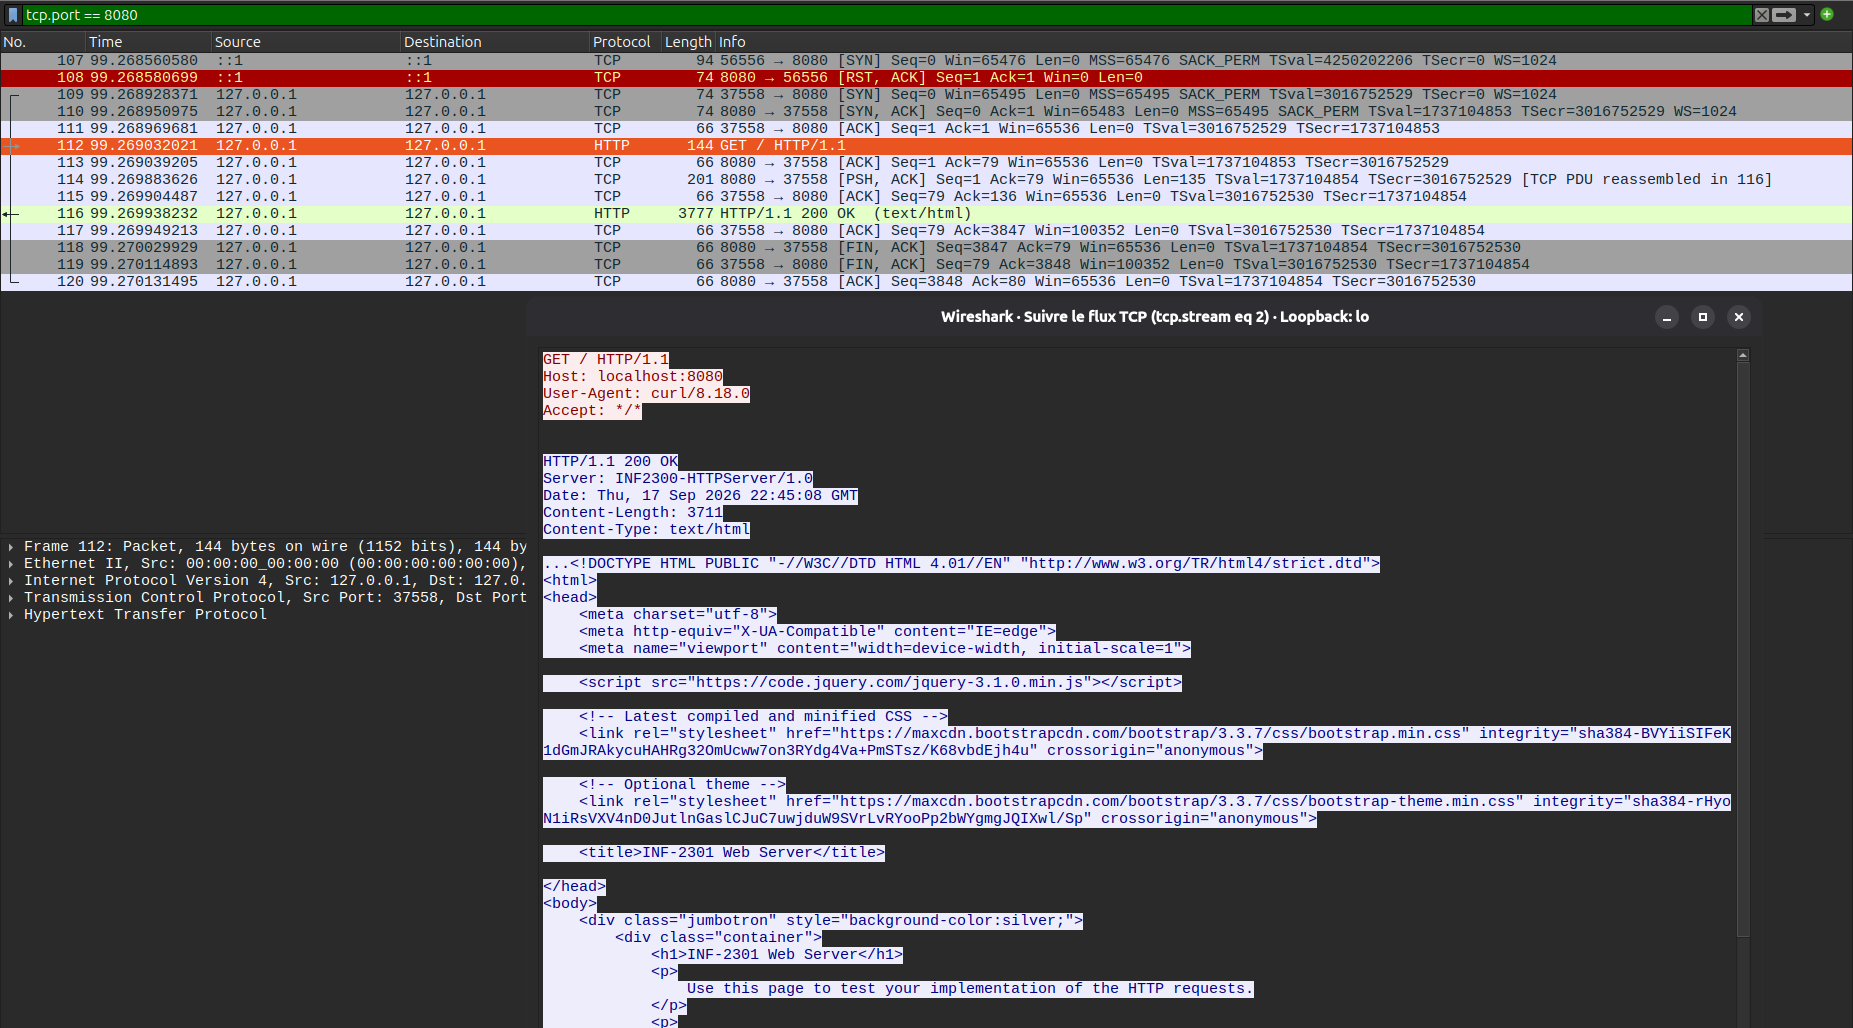
\includegraphics[width=\linewidth]{figures/capture_static.png}
	\caption{Wireshark capture of a \texttt{GET~/} request/response on the static file endpoint (loopback interface, \texttt{tcp.port == 8080}).}
	\label{fig:capture_static}
\end{figure}

\begin{figure}[htbp]
	\centering
	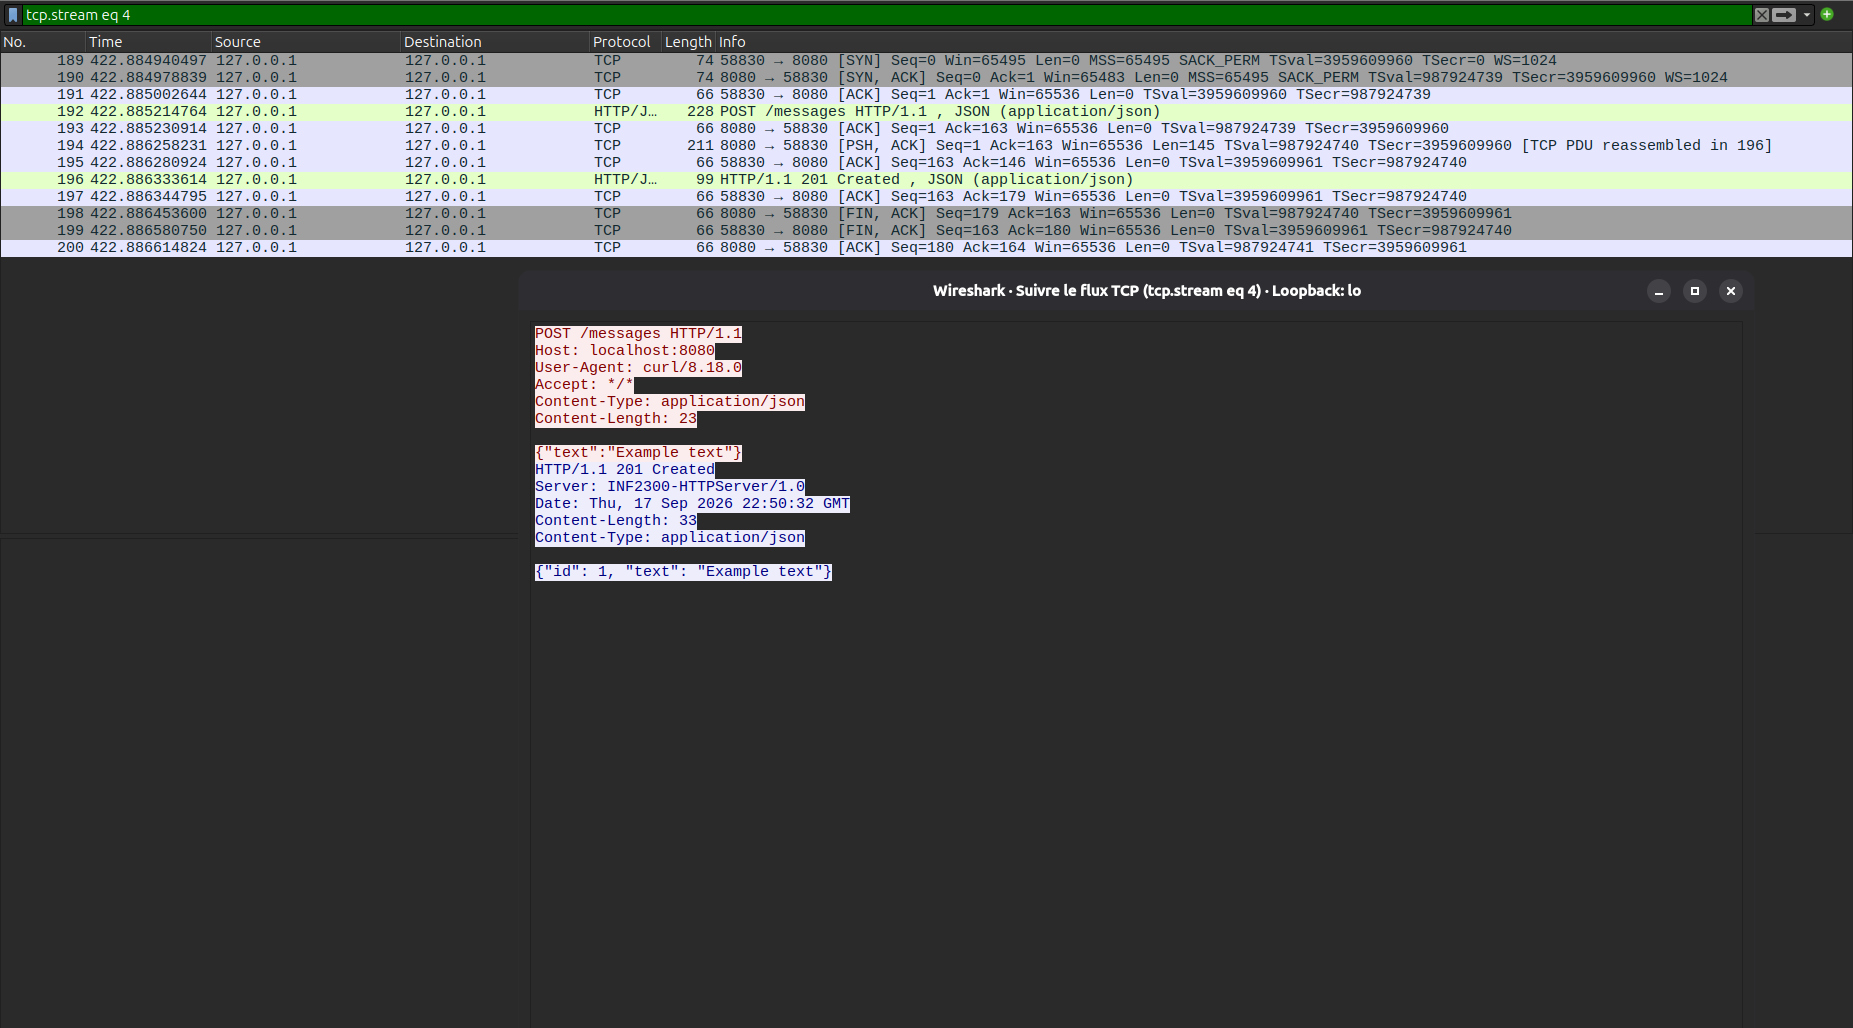
\includegraphics[width=\linewidth]{figures/capture_dynamic.png}
	\caption{Wireshark capture of a \texttt{POST~/messages} request/response on the REST endpoint, showing the JSON payload and the \texttt{201~Created} response.}
	\label{fig:capture_dynamic}
\end{figure}

\section{Discussion}\label{Section:Discussion}

\subsection{Unsupported and malformed methods}\label{Subsection:disc_unsupported}
A method outside \texttt{GET}/\texttt{POST}/\texttt{PUT}/\texttt{DELETE}
must not crash the server. This includes \texttt{HEAD} and a made-up verb
like \texttt{PIZZA}. I answer these with \texttt{501 Not Implemented},
rather than ignoring them or answering with \texttt{400}: the request line
is still valid HTTP, my server simply has no behaviour for that method,
which is exactly what \texttt{501} means. A structurally invalid request
is different, for example a request line without three fields, or a
header line without a colon. I answer these with \texttt{400 Bad Request},
since I cannot parse them as HTTP at all.

\subsection{Static file edge cases}\label{Subsection:disc_static}
A \texttt{POST} to any file other than \texttt{/test.txt}, such as
\texttt{server.py}, gets \texttt{403}: writability is opt-in, like
readability, and only \texttt{/test.txt} is on the writable whitelist. A
\texttt{GET} to \texttt{/test.txt} before it exists gets \texttt{404},
since the file genuinely does not exist yet. This differs from
\texttt{GET /messages}, which returns \texttt{200} with an empty array:
the \texttt{/messages} resource exists, it just has no content yet, while
\texttt{/test.txt} as a file does not exist until the first successful
\texttt{POST}. A directory traversal attempt, such as requesting
\texttt{/../README.md}, gets \texttt{403}, verified both by
\texttt{test\_client.py} and manually with \texttt{curl}. I prefer a
whitelist with a \texttt{realpath} containment check over blacklisting
patterns like \texttt{".."}: a blacklist has to anticipate every way to
manipulate a path, such as URL encoding or mixed separators, while
checking that the real path stays inside \texttt{BASE\_DIR} handles all
of them at once.

\subsection{/messages edge cases}\label{Subsection:disc_messages}
I ignore any \texttt{id} field a client sends in a \texttt{POST} body: the
server always assigns the id itself, since trusting a client-supplied id
could let one client overwrite a message it does not own. A \texttt{POST}
with no \texttt{text} field, or a \texttt{PUT} with an id but no
\texttt{text} field, gets \texttt{400}: these are malformed requests, not
missing resources. A \texttt{PUT} with no \texttt{id} at all also gets
\texttt{400}, not \texttt{404}, since the request itself is invalid,
independent of any id; this differs from a \texttt{PUT}/\texttt{DELETE}
with a valid id that simply does not exist, which gets \texttt{404}. An
empty body, or a body that is not valid JSON, also gets \texttt{400}.
Finally, a \texttt{POST} to \texttt{/messages/<id>} gets \texttt{403}:
creating a message at a URL for a specific, existing id does not make
sense, so only the collection endpoint, \texttt{/messages}, accepts new
messages.

\subsection{Security considerations}\label{Subsection:disc_security}
I apply the whitelist-over-blacklist choice from Section
\ref{Subsection:disc_static} as a general principle: a route or file that
is not explicitly listed is forbidden by default, so a new file added to
the project directory later is never exposed by accident. The directory
traversal test confirms this. I consider authentication and rate limiting
out of scope for this assignment.

\subsection{Persistence and crash safety}\label{Subsection:disc_persistence}
I write to a temporary file and then rename it into place, instead of
writing directly to \texttt{messages.json}: a crash during a direct write
could leave a truncated, unreadable JSON file, silently discarding every
earlier message. The atomic rename removes this risk entirely: at any
point, \texttt{messages.json} is either the old, complete state, or the
new, complete state. One limitation remains: I do not lock
\texttt{messages.json} against two simultaneous requests. This is
acceptable for the assignment's single-client testing model, but I note
it here as a known limitation.

\section{Conclusion}\label{Section:Conclusion}
This report presents an HTTP/1.1 server built on \texttt{socketserver},
exposing a static file endpoint and a persistent, RESTful
\texttt{/messages} endpoint through one generic request handler. The
solution meets the assignment's requirements. I verify it with two
automated test suites, 12/12 and 23/23, both passing in sequential and
random order, and with Wireshark packet captures. I implement three extra
credits: whitelist-based path traversal protection, \texttt{Server} and
\texttt{Date} headers, and \texttt{/messages/<id>} addressing. Two
limitations remain for future work: a locking mechanism for
\texttt{messages.json} under concurrent requests, and a real \texttt{3xx}
redirect from \texttt{/} to \texttt{/index.html}.

\section*{AI Usage Declaration}
\begin{itemize}
	\item \textbf{Tool used:} Claude Sonnet 5.1 (Anthropic), used through the
	Claude Code CLI.
	\item \textbf{Purpose of use:} I used the tool as an assistant while
	working on this assignment. I used it to discuss and refactor the design
	of the server's routing code, to write the two automated test suites, to
	set up the git repository, and to produce a first draft of the text in
	this report.
	\item \textbf{Author's declaration of responsibility:} I reviewed, tested,
	and edited all AI-assisted code and text before submitting this
	assignment. I take full responsibility for the correctness, originality,
	and content of the final code and report submitted here.
\end{itemize}

\printbibliography

\end{document}
